\section{Methods and Materials}\label{sec2}%Methods
\subsection{Participants}
15 participants (11- females and 4 males, mean age 23 $\pm$ 3 years) took part in the experiment.
They were informed about the relevant experimental procedures before providing their consent. Participants had no history of hearing disorder and had normal or corrected vision. The experimental procedures were approved by the ethics committee at Leipzig University. Monetary compensation was provided to the participants based on the time they spend at the experiment.

\subsection{Earmolds}
To alter participants’ perception of sound source elevation, their pinnae were consecutively modified by two sets of silicone molds. As a result, spectral cues derived from the shape of the external ears were changed sufficiently to diminish participants ability to locate sounds on the vertical axis. Earmolds were created by applying fast curing, skin safe silicone (SkinTite, Smooth-On, Macungie, USA) to the cymba conchae, cavum conchae and the antihelix while keeping the ear canal unobstructed [Fig. X]. Shape and volume of the earmolds varied between individuals to achieve similar degrees of disruption of vertical sound localization across participants. Two participants did not complete the experiment (first earmolds: n = 14, second earmolds: n = 13) and were removed from the analysis for these molds. 

\subsection{Experimental procedure}
The experiment was designed to adapt listeners to multiple sets of spectral cues for sound localization: participants wore two distinct pairs of earmolds consecutively (further denoted as molds 1 and molds 2), each over the course of a five-day adaptation period. The acoustical and behavioral impact of the molds were measured and the trajectories of participants’ adaptation throughout the following days were recorded to capture the occurrence of metaplasticity. To test whether learning a new set of spectral cues interferes with a previously learned mapping, the persistence of adaptation to the initial earmolds was measured after participants adapted to the second pair of molds for five days. This measurement was repeated for the second set of molds after five days without earmolds (see \cref{fig:adaptation}). During their first visit participants were familiarized with the environment, equipment and procedures of the free-field localization task. To minimize procedural learning during the experiment, participants completed at least one localization run and were free to continue practicing until they felt comfortable with the task. No feedback was given. After the initial familiarization, participants performed one localization task to measure their baseline localization accuracy. Once this task was completed, participants’ HRTFs were acquired. Participants’ ears were then modified by fitting the first pair of earmolds, before immediately repeating the localization task. To capture changes to spectral cues induced by the earmolds, another set of HRTFs was acquired. From that day on, the silicone molds were worn by the participants for five consecutive days. Throughout this adaptation period, participants underwent a daily routine of training sessions. Each training session was followed by a free-field localization task. On the final day of the first adaptation period (day 5 in \cref{fig:adaptation}), participants completed a short training session and a localization test. As a control, a subset of 6 participants performed an additional localization task presenting stimuli with varying spectral content in each trial. The earmolds were then removed, and participants’ localization accuracy was immediately measured again to test for aftereffects. The second pair of earmolds was then fitted to the participants’ ears, their initial localization accuracy was measured and HRTFs were acquired. Over the next 5 days, the procedure was repeated as described for the first adaptation period, including daily training sessions and localization tasks. After mold removal at the end of the second adaptation period (day 10 in \cref{fig:adaptation}), the first set of earmolds was briefly re-inserted and participants completed a localization run. To compare the persistence of adaptation to both sets of molds, participants returned to the lab after 5 days for a final localization test with the second molds re-inserted. The localization tests, binaural recordings and training sessions were conducted in a hemi-anechoic room (a x b x c m). Participants were seated in a comfortable chair in front of a spheric array of 45 loudspeakers (Mod1, Orb Audio, New York, USA) with a diameter of 1.4 m, covering the frontal hemisphere. Loudspeakers were hidden by an acoustically transparent black curtain to avoid visual cues of the sound source positions. Optionally, a small light emitting diode that was visible through the curtain indicating the central location of the frontal hemifield (0° Azimuth, 0° Elevation). During the localization tasks and training sessions, participants wore a headband with a laser pointer and an electromagnetic motion sensor (METAMOTIONRL, MBIENTLAB INC, San Francisco, USA) attached. The laser light was reflected by the curtain and provided visual feedback for the participants to indicate perceived sound source directions. Real time head orientation and position captured by the motion sensor were used to calculate azimuth and elevation of the participants’ response.

\subsection{Stimuli}
The stimuli used in the free-field localization task were 225 ms long sequences of pulsed pink noise, each composed of five equally spaced bursts of 25 ms duration. In the additional localization task, stimuli consisted of 225 ms long mixtures of environmental sounds. Each stimulus was composed of 6 randomly arranged excerpts of sounds drawn from a list of 42 recordings and had a unique spectrum. The Stimuli were re-generated on each trial and controlled by a custom python script using the slab toolbox \citep{schonwiesner_soundlab_2021}. Overall sound pressure level (SPL) of the stimuli at the position of the participants’ ears was 42 dB. Stimuli were processed digitally and amplified via TDT System 3 hardware (Tucker Davis Technologies, Alachua, USA). To minimize spectral localization cues independent of participant’s HRTFs, transfer functions for every loudspeaker  were measured by a probe microphone (Brüel \& Kjær, Nærum, Denmark) positioned at equal distance and orientation. A bank of inverse finite impulse response (FIR) filters was designed for each speaker to reduce differences in amplitude and frequency response across the loudspeakers. 

\subsection{Localization task} 
44 Loudspeakers were used for the localization task, covering 102° in azimuth (-52.5° to 52.5°) and 75° in elevation (-37.5° to 37-5°) of the hemisphere in front of the participant. Loudspeaker positions are described in an interaural-polar coordinate system. The loudspeakers were arranged on a spherical grid, formed by 7 loudspeakers on the horizontal and 7 loudspeakers on the vertical axis. Loudspeakers were distributed on the sphere with an angular distance of 17.5° in azimuth and 12.5° in elevation between neighboring speakers [Fig. X]. The 4 outermost loudspeakers (at +/- 52.5° azimuth and +/- 37.5° elevation) were excluded. At the beginning of each trial, participants were instructed to aim the head mounted laser at a centrally presented LED while pressing the button on a handheld box. When the button was pressed, participant’s initial head position was recorded and the stimulus was presented at a pseudorandom direction. Participants were instructed to indicate the perceived direction by turning their head towards the sound source and to confirm their response by pressing the button again. The horizontal and vertical angular displacement from the initial to the indicating head orientation was used to measure participant’s responses. No feedback was given. Each direction was presented three times during a localization run, with an angular distance of at least 35° between sound locations of two consecutive trials to reduce adaptation and assimilation \citep{ward_stimulus_1979}. 

\subsection{Training}
The training task was designed to accelerate the adaptation to new spectral cues and was introduced to participants as a game-like scenario. Participants were instructed to find the location of a pulsed pink noise played from one of the 44 speakers. Proprioceptive feedback was provided by varying pulse duration and the delay between the pulses depending on participant’s head orientation. Duration and delay of consecutive pulses decreased logarithmically with the angular distance between sound direction and the participant’s head direction, from up to 500 ms at 65° angular distance. (the maximal distance (52.5° in azimuth and 37.5° in elevation). The pulse train gradually merged into a continuous sound when participants directed the head mounted laser within 3° angular distance to the sound source. If participants remained oriented at the target area for at least 500 ms, the sound source was considered found and a popular video game sound was played as a reward signal. The target sound location was then switched at least 45° away from the previous one. Additionally, participants scored points for every found location and were rewarded more points if they located the sounds faster. Participants tried to score as many points as possible within 90 seconds. The final score was displayed on a screen after each round and a leaderboard encouraged competition amongst participants. Throughout the adaptation periods, participants underwent a daily routine of three 10-minute training sessions, intermitted by 5-minute breaks.

\begin{wrapfigure}[15]{r}{10cm}
\centering
\raisebox{0pt}[\dimexpr\height+1.6\baselineskip\relax]{
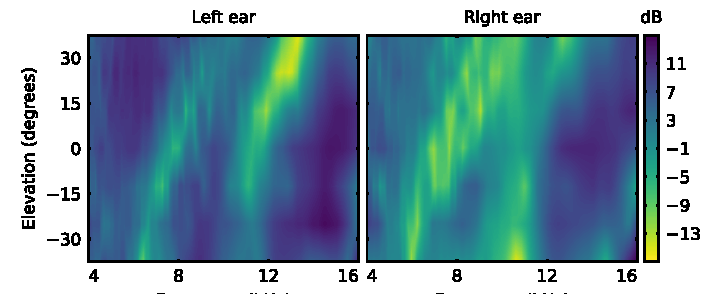
\includegraphics[width=10cm]{../Results/figures/fig1/fig1}}
\caption{DTFs across 7 elevations on the vertical midline obtained from one participant. Color maps show the spectral amplitude computed at 83 frequency bins between 4 and 16 kHz. The spectral profile was linearly interpolated between the measured DTFs for display.}
\label{fig:ef_l_r}
\end{wrapfigure}
\noindent%\vspace{-3\baselineskip}

\subsection{Directional transfer functions}
Binaural recordings were conducted to extract directional transfer functions (DTFs) of participant’s pinnae with and without silicone molds. PUM-3046L-R miniature microphones (PUIaudio, Fairborn, USA) were inserted in the ear canal to measure the sound pressure level at the ear eardrum. To minimize non-directional contributions by standing-wave pattern in the canal, the microphones were placed 2 mm into the entrance of the blocked ear canal. Participants were seated in front of the loudspeaker array and were asked to remain stationary during the measurement while aiming the head mounted laser at the central LED. Frequency modulated sweeps of 100 ms duration were presented 30 times from each of the 7 loudspeakers on the vertical midline (0° azimuth, -37.5° to 37.5° elevation). Repetitions were averaged for every location to increase signal to noise ratio. Recordings were digitized via TDT system 3 hardware at a sampling rate of 97 kHz. DTFs were extracted from the time-averaged recordings by taking the ratio of the Fourier transform of the acquired signal to the Fourier transform of the input signal. To remove non-directional portions of the transfer functions (such as ear canal and microphone transfer functions) each measured transfer function was divided by the grand average across the DTFs of all participants with and without molds (n = 588). To avoid over-representing higher frequencies, DTFs were processed with a bank of octave spaced cosine band-pass filters as proposed by \citet{middlebrooks_individual_1999}. Center frequencies were equally spaced at 0.0286 octaves between 4 and 16 kHz resulting in 2\% frequency difference between each of the 83 filters. The DTFs obtained from the left and right ear of one participant are shown in \cref{fig:ef_l_r}. Spectral information in participants' DTFs that could potentially guide vertical sound localization was quantified by measures introduced in previous studies. Vertical spectral information (VSI), VSI dissimilarity \citep{trapeau_fast_2016} and spectral strength \citep{andeol_sound_2013} were computed from DTFs obtained from the left and right ear. For comparison with behavioral measures left and right ear values were averaged.

\subsection{Statistical analysis}
Sound localization accuracy was quantified by the root mean square of the distance (RMSE) between the physical target and the perceived response locations for azimuth and elevation respectively. Horizontal and vertical variance of participant’s responses was quantified by taking the grand mean across standard deviations (SD) of the response coordinates for each sound location. The participant’s ability to perceive sound source elevation was additionally quantified by the elevation gain (EG), as the slope of the linear regression lines between target and response elevations \citep{hofman_relearning_1998}. Throughout the analysis, paired comparisons were statistically assessed using Wilcoxon signed-rank tests. Relations between measures were determined using Spearman correlation coefficients, p-values smaller than 0.05 were regarded as significant.
